\chapter{Introduction}
    %\addcontentsline{toc}{chapter}{\protect\numberline{}Introduction}
    
     % Might be useful: http://www.emerson.emory.edu/services/latex/latex_162.html

\section{General context}

%\section{Motivation}

%\section{Lean-premixed systems for pollutant reduction}
\section{Lean combustion in gas turbines}


\section{Fuel injection technology}

\begin{figure}[h!]
	\centering
	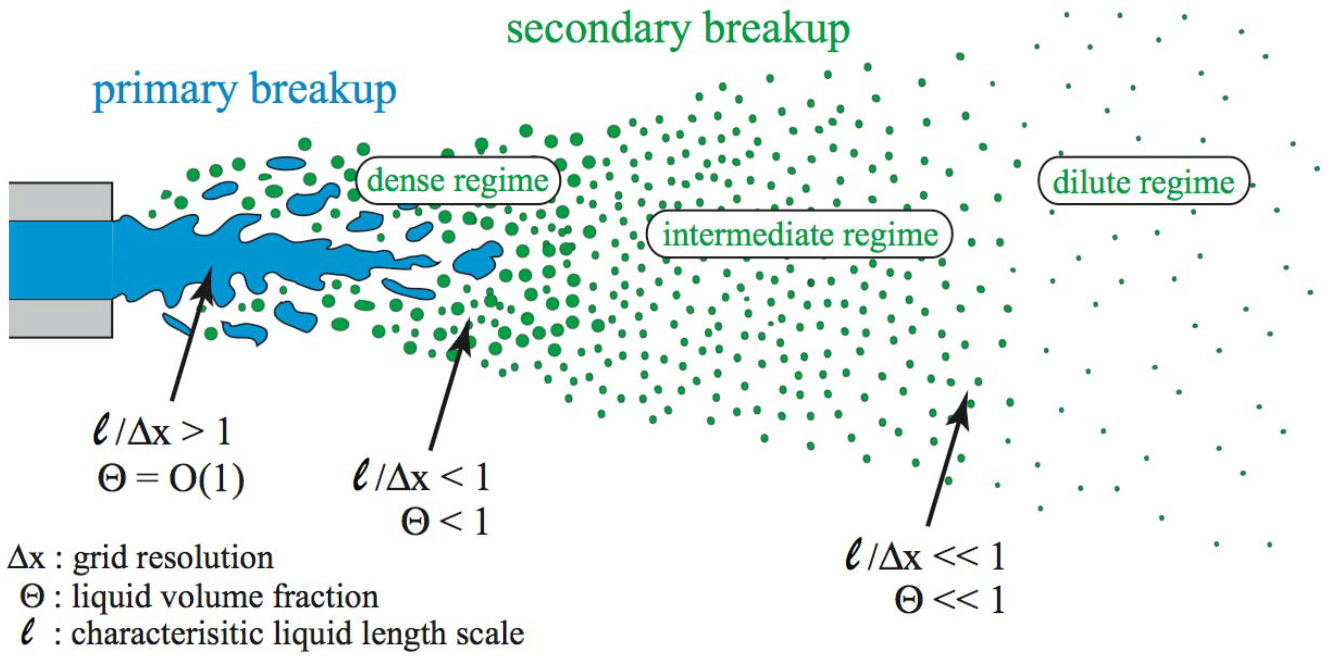
\includegraphics[scale=0.5]{./part0_intro/figures_intro/atomization-regimes-scheme}
	\caption{Atomization breakup regimes \citepColor[herrmann_modeling_2003]}
	\label{fig:atomization_regimes_herrmann}
\end{figure}

\subsection*{Atomization process}

Explain two-phase flows phenomenology (injection + atomization) here. 

Explain airblast, hollow-cone, jicf.

\section{Objective and thesis outline}
    %\addcontentsline{toc}{section}{\protect\numberline{}Manuscript organisation}

